\section{Acceso al Sistema (Login y Tablero)}

El acceso al sistema integrado Odoo SaaS de Textiles y Confecciones Atlas E.I.R.L. se realiza a través de un navegador web estándar. 

\subsection{Pantalla de Inicio de Sesión (Login)}

Para ingresar al sistema, debe dirigirse a la URL proporcionada por la administración. En esta pantalla, se le solicitará su correo electrónico institucional y su contraseña personal, la cual es de uso intransferible y confidencial.

\begin{figure}[H]
    \centering
    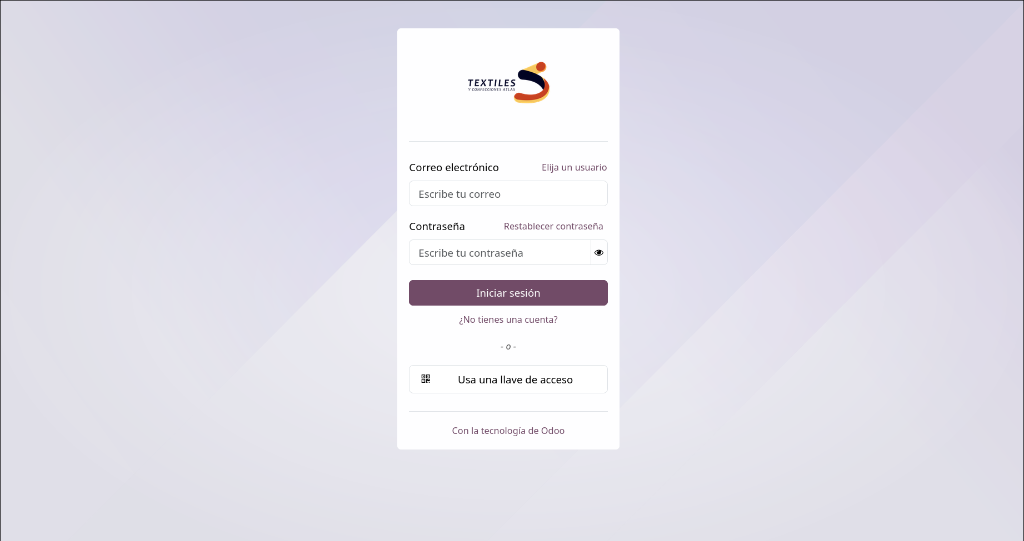
\includegraphics[width=0.85\textwidth]{assets/login.png}
    \caption{Pantalla de inicio de sesión de Odoo.}
\end{figure}

Pasos para el ingreso:
\begin{enumerate}
    \item Escriba su \textbf{Correo electrónico}.
    \item Ingrese su \textbf{Contraseña}.
    \item Haga clic en el botón morado \textbf{Iniciar sesión}.
\end{enumerate}

\subsection{Tablero Principal (Dashboard)}

Una vez que las credenciales son validadas, el sistema lo dirigirá al Tablero Principal. Esta pantalla es el punto de partida hacia todas las aplicaciones y módulos habilitados para el control comercial y logístico de la empresa.

\begin{figure}[H]
    \centering
    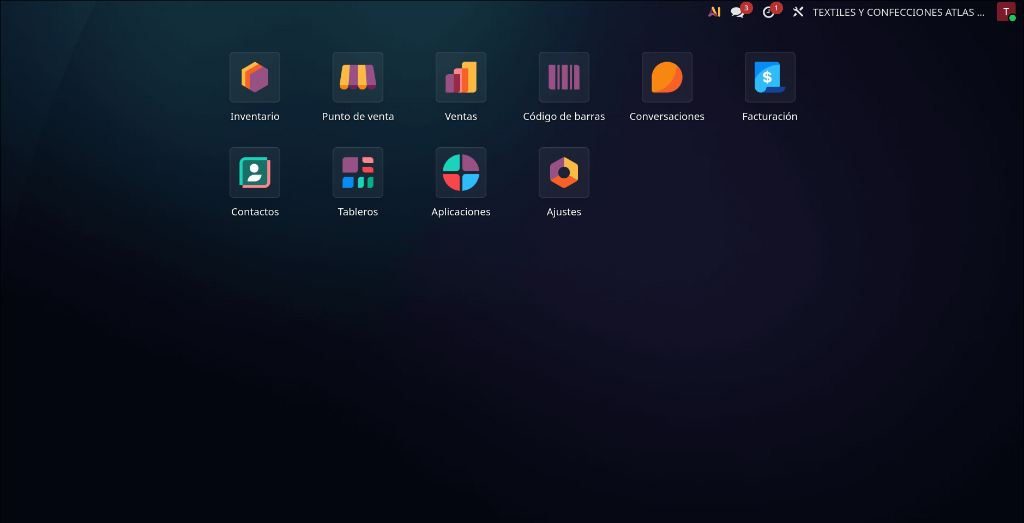
\includegraphics[width=0.85\textwidth]{assets/dashboard.png}
    \caption{Tablero Principal (Dashboard) con los módulos instalados.}
\end{figure}

Dependiendo de sus permisos de usuario, visualizará los siguientes módulos clave:
\begin{itemize}
    \item \textbf{Inventario:} Para gestionar existencias, ingresos y salidas de artículos deportivos.
    \item \textbf{Punto de Venta:} Para ejecutar las ventas rápidas en el mostrador de la tienda.
    \item \textbf{Contactos:} Directorio digital de clientes y proveedores.
    \item \textbf{Facturación / Ventas:} Para la gestión comercial y comprobantes.
\end{itemize}
